\documentclass[../main.tex]{subfiles}



\begin{document}




\chapter{Compacitat}
\section{Recobriments i subrecobriments}

\begin{defi}
[Recobriments]\label{def:recobriment}\label{def:subrecobriment}\index{Recobriment}\index{Subrecobriment} Sigui $X$ un espai topològic i $A\subseteq X$. Un \textit{recobriment d'$A$} és una col·lecció de subconjunts $\mathcal{F}$ de $X$ tal que
\begin{equation}
    \notag
    A\subseteq \bigcup_{U\in\mathcal{F}}U.
\end{equation}
Si $\mathcal{F}$ és una col·lecció d'oberts, aleshores es diu recobriment obert. Anàlogament, si $\mathcal{F}$ és una col·lecció de tancats, es diu recobriment de tancats. Si $\mathcal{F}^*\subseteq\mathcal{F}$ també cobreix $A$, es diu que $\mathcal{F}^*$ és un \textit{subrecobriment d'$A$ de $\mathcal{F}$}. Un \textit{recobriment de tot l'espai $X$} és una família de subconjunts $\{X_\gamma\}_{\gamma\in\Gamma}$ tals que
\begin{equation}
    \notag
    X = \bigcup_{\gamma\in \Gamma}X_\gamma.
\end{equation}
\end{defi}

\begin{ej}
\label{ej:recobriment1} Una base forma un recobriment obert de tot l'espai. Prenent l'adherència de cada element del recobriment obtenim un recobriment tancat.
\end{ej}

\begin{ej}
\label{ej:recobriment2} Considerem l'espai topològic $\mathbb{R}$ amb la topologia usual. Considerem $A = \mathbb{N}\subseteq\mathbb{R}$. Tot singletó de $\mathbb{R}$ és tancat i per tant la col·lecció
\begin{equation}
    \notag
    \{\{n\}\;:\;n\in\mathbb{N}\}
\end{equation}
és un recobriment tancat de $\mathbb{N}$ ja que $\mathbb{N}= \bigcup_{n\in\mathbb{N}}\{n\}$. D'altra banda, la col·lecció 
\begin{equation}
    \notag
    \left\{\left(n-\frac{1}{2},n+\frac{1}{2}\right)\;:\;n\in\mathbb{N}\right\}
\end{equation}
és un recobriment obert de $\mathbb{N}$ ja que cada conjunt en aquesta família és un interval obert centrat en $n$ i de radi $1/2$ i
\begin{equation}
    \notag
    \mathbb{N}\subseteq \bigcup_{n\in\mathbb{N}}\left(n-\frac{1}{2},n+\frac{1}{2}\right).
\end{equation}
\end{ej}

\begin{ej}
\label{ej:recobriment3} Considerem $A = [0,1)\subset\mathbb{R}$. Aleshores, la col·lecció $\mathcal{F} = \{(-1,2/3),(1/2,2)\}$ és un recobriment obert de $[0,1)$.
\end{ej}

Recordem la construcció següent de la teoria de conjunts. Siguin $X,Y$ dos conjunts i sigui $f:X\rightarrow Y$ una aplicació. Si $\{X_\gamma\}_{\gamma\in \Gamma}$ és un recobriment de $X$, les restriccions $f_\gamma:X_\gamma\rightarrow Y$ verifiquen
\begin{equation}
    \notag
    f_{\gamma|X_\gamma\cap X_{\gamma'}} = f_{\gamma'|X_\gamma\cap X_{\gamma'}},\quad \forall \gamma,\gamma'\in \Gamma 
\end{equation}
i, recíprocament, donades aplicacions $\{f_\gamma\}_{\gamma\in\Gamma}$, $f_\gamma:X_\gamma\rightarrow Y$ que verifiquen les condicions anteriors, existeix una única aplicació de conjunts $f:X\rightarrow Y$ tal que $f_\gamma$ és $f_{|X_\gamma}$, per a tot $\gamma\in\Gamma$. Les construccions que buscàvem per construir aplicacions contínues són les següents:
\begin{prop}
\label{prop:recobrimentsiappcontinues} Siguin ara $X,Y$ espais topològics. Amb la mateixa notació, suposem $f_\gamma$ contínua per a tot $\gamma\in\Gamma$. Aleshores
\begin{enumerate}[(1)]
    \item Si el recobriment és tancat i finit, $f$ és contínua.
    \item Si el recobriment és obert, $f$ és contínua.
\end{enumerate}
\end{prop}
\begin{proof}
\begin{enumerate}[(1)]
    \item Sigui $T$ un tancat de $Y$. Aleshores
    \begin{equation}
        \notag
        f^{-1}(T) = \bigcup_{\gamma\in\Gamma}(f^{-1}(T)\cap X_\gamma) = \bigcup_{\gamma\in\Gamma}f_\gamma^{-1}(T)
    \end{equation}
    Com que $f_\gamma^{-1}(T)$ és un tancat de $X_\gamma$, que és tancat de $X$, $f_\gamma^{-1}(T)$ és tancat de $X$ i $f^{-1}(T)$, en ser reunió finita de tancats, és tancat.
    \item Sigui $U$ obert de $Y$. Aleshores
    \begin{equation}
        \notag
        f^{-1}(U)=\bigcup_{\gamma\in\Gamma}(f^{-1}(U)\cap X_\gamma) = \bigcup_{\gamma\in\Gamma}f_\gamma^{-1}(U).
    \end{equation}
    Com que $f_\gamma^{-1}(U)$ és un obert de $X_\gamma$ i $X_\gamma$ és obert, tenim que $f_\gamma^{-1}(U)$ és un obert de $X$. Així, $f^{-1}(U)$ és reunió d'oberts i per tant és un obert.
\end{enumerate}
\end{proof}

\begin{nota}
En cas d'un recobriment tancat la condició de finitud és una condició necessària. Per exemple, siguin $X = [0,1], X_n = \left[\frac{1}{n+1},\frac{1}{n}\right]$, amb $n>0$, i $X_\infty = \{0\}$. Sigui $f:X\rightarrow\mathbb{R}$ l'aplicació identitat a $(0,1]$ i $f(0) = 1$. Aquesta aplicació no és contínua i, en canvi, fa $f_n = f_{|X_n}$, $f_\infty = f_{|X_\infty}$ són contínues i $f_{n|X_n\cap X_m} = f_{m|x_n\cap X_m}$ per a tot $n,m\in\mathbb{N}\cup\{\infty\}$.
\end{nota}

\section{Espais quasi-compactes}
\subsection{Espais quasi-compactes}

\begin{defi}
[Quasi-compacte]\label{def:quasicompacte}\index{Espai quasi-compacte}\index{Quasi-compacte} Sigui $(X,\tau)$ un espai topològic. Diem que $X$ és \textit{quasi-compacte} si per a tot recobriment obert $\{U_i\}_{i\in I}$ de $X$ existeix un subrecobriment finit, és a dir, un subconjunt $J\subset I$ finit tal que $\{U_j\}_{j\in J}$ és un recobriment.
\end{defi}

Caracteritzem ara els subconjunts d'un espai topològic $X$ compactes. Si $X$ és un espai topològic i $A\subseteq X$ és un subconjunt dotat de la topologia subespai, quan és $A$ quasi-compacte?

\begin{prop}
\label{prop:subconjuntqc} Si $X$ és un espai topològic i $A\subseteq X$ un subespai topològic amb la topologia induïda per la inclusió, aleshores $A$ és compacte si i només si per tota col·lecció d'oberts $\{U_i\}_{i\in I}$ tals que $A\subseteq\bigcup_{i\in I}U_i$ existeix un conjunt finit $\{i_1,\ldots,i_n\}\subset I$ tal que $A\subseteq \bigcup_{j=1}^n U_{i_j}$.
\end{prop}
\begin{proof}
\begin{itemize}
    \item \fbox{$\Rightarrow$} $A$ és compacte si $\forall\{U_i\}_{i\in I}$ tal que $A = \bigcup_{i\in I}U_i$ (és a dir, per tot recobriment d'$A$) $\exists\{i_1,\ldots,i_n\}\subset I$ tal que $A = \bigcup_{k=1}^n U_{i_k}$. 
    
    Ara, si $\{U_i\}_{i\in I}$ és un recobriment obert d'$A$, $\forall i\in I$ $U_i$ és obert d'$A$ amb la topologia subespai. Per tant, $\exists W_i$ obert de $X$ tal que $U_i = W_i\cap A$. D'aquesta manera
    \begin{equation}
        \notag
        A = \bigcup_{i\in I}U_i = \bigcup_{i\in I}(W_i\cap A)\Longrightarrow A\subseteq \bigcup_{i\in I}W_i
    \end{equation}
    Més enllà, per la hipòtesis de compacitat de $A$, existeix un conjunt d'índexs finit $\{i_1,\ldots,i_n\}\subset I$ tal que $U_{i_1},\cdots,U_{i_n}$ és un recobriment obert de $A$. Així doncs, existiran oberts de $X$, $\{W_{i_1},\ldots,W_{i_n}\}\subset\{W_i\}_{i\in I}$ tals que $U_{i_k} = W_{i_k}\cap A$ i així obtenim que $A\subseteq\bigcup_{k=1}^n W_{i_k}$.
    \item \fbox{$\Leftarrow$} Suposem que es compleix que $\forall\{U_i\}_{i\in I}$ col·lecció d'oberts de $X$ tals que $A\subseteq \bigcup_{i\in I}U_i$ existeix $\{i_1,\ldots,i_n\}\subset I$ tal que $A\subseteq\bigcup_{k=1}^n U_{i_k}$. Aleshores, prenem un recobriment obert d'$A$, $\{V_i\}_{i\in I}$ de forma que $A = \bigcup_{i\in I}V_i$. Escollim $\forall i$ un obert $U_i$ de $X$ tal que $V_i = U_i\cap A$. D'aquesta manera, per hipòtesis
    \begin{equation}
        \notag
        A\subseteq \bigcup_{i\in I}U_i\Longrightarrow \exists J\subset I,\;|J|<\infty,\;tq\;A=\bigcup_{j\in J} V_j.
    \end{equation}
    D'aquesta manera obtenim que $A$ és compacte.
\end{itemize}
\end{proof}

Tot això ho fem motivats pel teorema de Heine-Borel d'anàlisi, que diu que un conjunt tancat i acotat de $\mathbb{R}$ admet, per a tot recobriment obert, un subrecobriment finit. Aquest teorema el demostrarem al final d'aquest capítol.

\begin{ej}
\label{ej:qc1} Pel teorema esmentat de Heine-Borel, tot subconjunt tancat i acotat de $\mathbb{R}$ és quasi-compacte. En particular, tot interval $[a,b]$, $a<b$, $a,b\in\mathbb{R}$ és quasi-compacte. Més en general, si $X = \mathbb{R}^n$ amb la topologia usual, aleshores $A\subset X$ és compacte si i només si és tancat i acotat. Això més tard ho veurem millor.
\end{ej}

\begin{ej}
\label{ej:qc2} Un espai topològic finit és quasi-compacte.
\end{ej}

\begin{ej}
\label{ej:qc3} Un conjunt infinit amb la topologia discreta no és quasi-compacte, ja que el recobriment obert donat pels punts no té un subrecobriment finit.
\end{ej}

\begin{coro}
[Exemple]\label{ej:qc4} $\mathbb{N}$ no és quasi-compacte en $\mathbb{R}$ (amb la topologia usual).
\end{coro}
\begin{proof}
Considerem el següent recobriment obert de $\mathbb{N}$:
\begin{equation}
    \notag
    \mathcal{F}=\left\{\left(n-\frac{1}{2},n+\frac{1}{2}\right)\;:\;n\in\mathbb{N}\right\} .
\end{equation}
Aleshores, cada element de $\mathcal{F}$ conté exactament un nombre natural i la col·lecció $\mathcal{F}$ conté un nombre numerable però infinit d'elements. Si $\mathcal{F}^*\subseteq\mathcal{F}$, aleshores $\mathbb{N}\not\subset \bigcup_{I\in\mathcal{F}^*} I$, ja que $\mathcal{F}^*\subseteq \mathbb{F}$ és finit implica que existeix alguna $n\in\mathbb{N}$ que no està continguda a cap conjunt de $\mathcal{F}^*$ i per tant $\mathcal{F}^*$ no és un recobriment.
\end{proof}

\subsection{Quasi-compacitat de conjunts finits}

A l'exemple 2 (\ref{ej:qc2}) hem vist que tot espai topològic finit és quasi-compacte. Ara intentarem provar aquest fet, provant abans que tot subconjunt finit d'un espai topològic és quasi-compacte.

\begin{prop}
\label{prop:subconjuntfinitqc} Sigui $X$ un espai topològic qualsevol. Si $A\subseteq X$ és un subconjunt finit, aleshores és quasi-compacte en $X$.
\end{prop}
\begin{proof}
Sigui $A\subseteq X$ un conjunt finit. Sigui, per exemple, $A = \{x_1,\ldots,x_n\}$. Sigui $\mathcal{F}=\{A_i\;:\;i\in I\}$ un recobriment obert d'$A$. Així
\begin{equation}
    \notag
    A\subseteq \bigcup_{i\in I}A_i.
\end{equation}
Com $\mathcal{F}$ recobreix $A$, el conjunt $A$ pot ser partit en com a màxim $n$ grups d'elements d'$A$ on cada element d'aquests grups està contingut en algun $A_i\in\mathcal{F}$, $i\in I$. Per tant, existeix una subcol·lecció $I^*\subseteq I$ tal que 
\begin{equation}
    \notag
    A\subseteq \bigcup_{i\in I^*}A_i,
\end{equation}
a més $|I^*|\leq n$. Per tant,
\begin{equation}
    \notag
    \mathcal{F}^*=\{A_i\;:\;i\in I^*\}
\end{equation} és un subrecobriment finit de $A$.
\end{proof}

\begin{coro}
\label{coro:totespaifinitesqc} Tot espai topològic $X$ finit és quasi-compacte.
\end{coro}
\begin{proof}
Per la proposició, com tot subconjunt $A\subseteq X$ és finit, aleshores és quasi-compacte. Així $X$ és quasi-compacte.
\end{proof}

\subsection{Propietat de la intersecció finita}

En aquest apartat donaré una definició equivalent de subconjunt quasi-compacte, en forma de teorema. Als apunts del Naranjo-Navarro surt com una definició alternativa, però jo ho entenc millor així.

\begin{ter}
\label{ter:defalternativadeqc} Sigui $X$ un espai topològic. Aleshores $X$ és quasi-compacte si, i només si, per a tota col·lecció $\mathcal{F}$ de tancats de $X$ satisfent que tota subcol·lecció finita de $\mathcal{F}$, $\{F_1,\ldots,F_n\}\subset\mathcal{F}$ compleix que $\bigcap_{i=1}^n F_i\not=\emptyset$, satisfà
\begin{equation}
    \notag
    \bigcap_{F\in\mathcal{F}} F\not=\emptyset
\end{equation}
\end{ter}
\begin{proof}
\begin{itemize}
    \item \fbox{$\Rightarrow$} Suposem que $X$ és compacte. Sigui $\mathcal{F}$ una família de tancats de $X$ tal que tota subfamília finita $\{F_1,\ldots,F_n\}$ de $\mathcal{F}$ satisfà
    \begin{equation}
        \notag
        \bigcap_{i=1}^n F_i\not=\emptyset.
    \end{equation}
    Hem de veure que $\bigcap_{F\in\mathcal{F}}\not=\emptyset$. Suposem que no, és a dir, que aquesta intersecció és buida. Prenent complementaris,
    \begin{equation}
        \notag
        \left(\bigcap_{F\in\mathcal{F}}F\right)^c = \emptyset^c \Leftrightarrow \bigcup_{F\in\mathcal{F}}F^c = X.
    \end{equation}
    Com $F$ és tancat, $\forall F\in\mathcal{F}$, $F^c$ és obert. Per tant, $\{F^c\;:\;F\in\mathcal{F}\}$ és un recobriment obert de $X$. Com $X$ és compacte, existeix un subrecobriment finit, sigui $\{F_1^c,\ldots,F_n^c\}\subseteq\{F^c\;:\;F\in\mathcal{F}\}$ tal que
    \begin{equation}
        \notag
        \bigcup_{i=1}^n F_i^c = X.
    \end{equation}
    Tornant als complementaris
    \begin{equation}
        \notag
        \left(\bigcup_{i=1}^n F_i^c\right)^c = X^c\Leftrightarrow \bigcap_{i=1}^n F_i = \emptyset
    \end{equation}
    cosa que contradiu la hipòtesis inicial.
    \item \fbox{$\Leftarrow$} Suposem que $X$ no és compacte i prenent complementaris s'arriba de manera anàloga a una contradicció.
\end{itemize}
\end{proof}

\section{Propietats dels espais quasi-compactes}
\subsection{Tancats a espais quasi-compactes}

\begin{prop}
\label{prop:tancatesqc} Sigui $X$ un espai topològic quasi-compacte i sigui $A\subseteq X$. Si $A$ és tancat, aleshores $A$ és quasi-compacte.
\end{prop}
\begin{proof}
Sigui $\mathcal{F} = \{A_i\}_{i\in I}$ un recobriment obert de $A$. Aleshores,
\begin{equation}
    \notag
    A\subseteq \bigcup_{i\in I} A_i.
\end{equation}
Com $A$ és tancat, $A^c$ és obert. Notem que $\{A_i\}_{i\in I}\cup\{A^c\}$ és un recobriment obert de tot $X$. Com $X$ és un espai quasi-compacte, existeix un subrecobriment finit obert $\{A_1,\ldots,A_n\}\cup\{A^c\}$ tal que
\begin{equation}
    \notag
    X\subseteq\left(\bigcup_{i=1}^n A_i\right)\cup(A^c)
\end{equation}
però aleshores $\{A_1,\ldots,A_n\}$ és un subrecobriment finit de $A$, ergo $A$ és quasi-compacte en $X$.
\end{proof}

\subsection{Conjunts quasi-compactes a espais de Hausdorff}

A l'apartat anterior hem vist que si $X$ és un espai topològic quasi-compacte i $A\subseteq X$, aleshores $A$ tancat implica $A$ quasi-compacte. Ara veurem que si $X$ és de Hausdorff, aleshores se satisfà la implicació recíproca.

\begin{prop}
\label{prop:ent2qcimplicatancat} Sigui $X$ un espai topològic de Hausdorff i $A\subseteq X$. Si $A$ és quasi-compacte en $X$, aleshores és tancat.
\end{prop}
\begin{proof}
Sigui $A$ un conjunt quasi-compacte en $X$. Sigui $y\in A^c$ un punt fix. Com $X$ és un espai de Hausdorff, i la propietat de Hausdorff és hereditària 
(\ref{prop:hausdorff2}), $A$ també és de Hausdorff. Aleshores, $\forall x\in A$, $\exists U_x$ entorn obert de $x$ i $V_{(y,x)}$ de $y$ tals que
\begin{equation}
    \notag
    U_x\cap V_{(y,x)} = \emptyset.
\end{equation}
Aleshores tenim que $\{U_x\}_{x\in A}$ és un recobriment obert d'$A$. Com $A$ és quasi-compacte, existeix un subrecobriment finit $\{U_{x_1},\ldots,U_{x_n}\}$ on $x_i\in A$, $\forall i\in\{1,\ldots,n\}$ i 
\begin{equation}
    \notag
    A\subseteq \bigcup_{i=1}^n U_{x_i}.
\end{equation}
Corresponentment, el conjunt $\{V_{(y,x_1)},\ldots,V_{(y,x_n)}\}$ d'entorns oberts tals que
\begin{equation}
    \notag
    U_{x_i}\cap V_{(y,x_i)} = \emptyset,\quad \forall i\in\{1,\ldots,n\} .
\end{equation}
Sigui
\begin{equation}
    \notag
    V\equiv \bigcap_{i=1}^n V_{(y,x_i)}.
\end{equation}
Aleshores, $V$ és una intersecció finita d'oberts i per tant és obert. A més, $V$ és un entorn obert de $y$. Addicionalment, $A\cap V = \emptyset$ ja que $\bigcup_{i=1}^n U_{x_i}$ recobreix $A$. Com $A\cap V = \emptyset$ això implica que $V\subseteq A^c$. Aleshores $V$ és un entorn obert de $y$, que està contingut totalment en $A^c$, és a dir, $y\in(A^c)^{o}$. Per tant $(A^c)^{o} = A^c\Rightarrow A$ és tancat.
\end{proof}

\subsection{Preservació de la quasi-compacitat per aplicacions contínues}

\begin{prop}
\label{prop:preservaciodelaqcperappcontinues} Sigui $f:X\rightarrow Y$ una aplicació contínua i exhaustiva (aquesta condició es pot canviar dient $f:X\rightarrow Y$ contínua i que si $X$ és compacte aleshores $f(X)$, el conjunt imatge, és compacte en $Y$. Més en general, si $A\subseteq X$ és compacte en $Y$, no cal l'exhaustivitat) entre espais topològics. Si $X$ és quasi-compacte, aleshores $Y$ també ho és.
\end{prop}
\begin{proof}
Sigui $\{U_i\}_{i\in I}$ un recobriment obert de $Y$. Aleshores $\{f^{-1}(U_i)\}_{i\in I}$ és un recobriment obert de $X$ i, per tant, existeix $J\subseteq I$ finit tal qeu 
\begin{equation}
    \notag
    X = \bigcup_{i\in J}f^{-1}(U_i).
\end{equation}
Així, com $f$ és exhaustiva, $Y = \bigcup_{i\in J}U_i$.
\end{proof}

\begin{prop}
\label{prop:qchausdorff} Sigui $X$ i $Y$ dos espais topològics i $f:X\rightarrow Y$ una aplicació contínua i bijectiva. Si $X$ és quasi-compacte i $Y$ és de Hausdorff, aleshores $f$ és un homeomorfisme.
\end{prop}
\begin{proof}
Com $f$ ja és contínua i bijectiva d'hipòtesis, només queda veure que $f^{-1}$ és contínua. Això és, veure que per a qualsevol obert $U$ de $X$, $(f^{-1})^{-1}(U)$ és obert en $Y$ (equivalentment, que $f$ és oberta).

Sigui $U$ un obert de $X$. Aleshores $U^c$ és tancat en $X$ i com $X$ és quasi-compacte, $U^c$ és també quasi-compacte. Per la proposició anterior (\ref{prop:preservaciodelaqcperappcontinues}) $f(U^c)$ és quasi-compacte, i per la proposició (\ref{prop:ent2qcimplicatancat}), com $Y$ és de Hausdorff, $f(U^c)$ és tancat en $Y$. Finalment $f(U^c) = f(U)^c$ que és tancat i aleshores $(f(U)^c)^c = f(U)$ és obert com volíem veure.
\end{proof}

\begin{lema}
\label{lema:qchausdorfftapptancada} Sigui $X$ un espai topològic quasi-compacte i $Y$ un espai topològic de Hausdorff, i sigui $f:X\rightarrow Y$ contínua. Aleshores $f$ és tancada.
\end{lema}
\begin{proof}
Sigui $C$ un tancat en $X$. Per la proposició (\ref{prop:tancatesqc}) $C$ és quasi-compacte en $X$ i per la proposició (\ref{prop:preservaciodelaqcperappcontinues}) com $f$ és contínua, $f(C)$ és quasi-compacte en $Y$. Per la proposició (\ref{prop:ent2qcimplicatancat}) tot quasi-compacte en un espai $T_2$ és tancat, per tant $f(C)$ és tancat.
\end{proof}





\subsection{Quocients a espais quasi-compactes}

\begin{ter}
\label{ter:quocientqc} Siguin $X$ i $Y$ espais topològics i $f:X\rightarrow Y$. Si $X$ és quasi-compacte, $Y$ de Hausdorff i $f$ contínua i exhaustiva, aleshores si $\sim_f$ és la relació d'equivalència definida com $x\sim_f y\Leftrightarrow f(x)=f(y)$, tenim que $X/\sim_f\cong Y$.
\end{ter}
\begin{proof}
Del lema (\ref{lema:qchausdorfftapptancada}) veiem que com $X$ és compacte, $Y$ de Hausdorff i $f$, contínua, que $f$ és una aplicació tancada. Com, a més, és exhaustiva, $f(X) = Y$. Pel teorema (\ref{ter:topologiaquocientobert}) $X/\sim_f\cong f(X) = Y$.
\end{proof}

\section{Productes i espais quasi-compactes}
\subsection{El lema del tub}

Per tractar el producte d'espais quasi-compactes necessitem un resultat previ.

\begin{lema}
[Lema del tub]\label{lema:lemadeltub} Sigui $X$ un espai topològic i sigui $Y$ un espai topològic quasi-compacte. Per a tot punt $x_0\in X$ i per a tot entorn $E$ de $\{x_0\}\times Y$ a $X\times Y$, existeix un entorn obert $U$ de $x_0$ a $X$ tal que $U\times Y\subset E$.
\end{lema}
\begin{proof}
Utilitzant que els oberts de la forma $U\times V$ formen base (recordem de (\ref{defi:topologiaproducte})) obtenim que, per a tot $y\in Y$, existeixen oberts $U_y$ de $X$ i $V_y$ de $Y$ tal que 
\begin{equation}
    \notag
    (x_0,y)\in U_y\times V_y\subset E.
\end{equation}
Aleshores $\{V_y\}_{y\in Y}$ formen un recobriment de $Y$. Per la quasi-compacitat existeixen $y_1,\ldots,y_n\in Y$ tals que $Y = V_{y_1}\cup\cdots\cup V_{y_n}$. Sigui $U = U_{y_1}\cup\cdots\cup U_{y_n}$ un entorn obert de $x_0$. Tenim que si $(x,y)\in U\times Y$ aleshores existeix $j\in\{1,\ldots,n\}$ tal que $y\in V_j$. Així 
\begin{equation}
    \notag
    (x,y)\in U\times V_j\subset U_v\times V_j\subset E.
\end{equation}
Per tant $U\times Y\subset E$.
\end{proof}

\begin{equation}
    \notag
    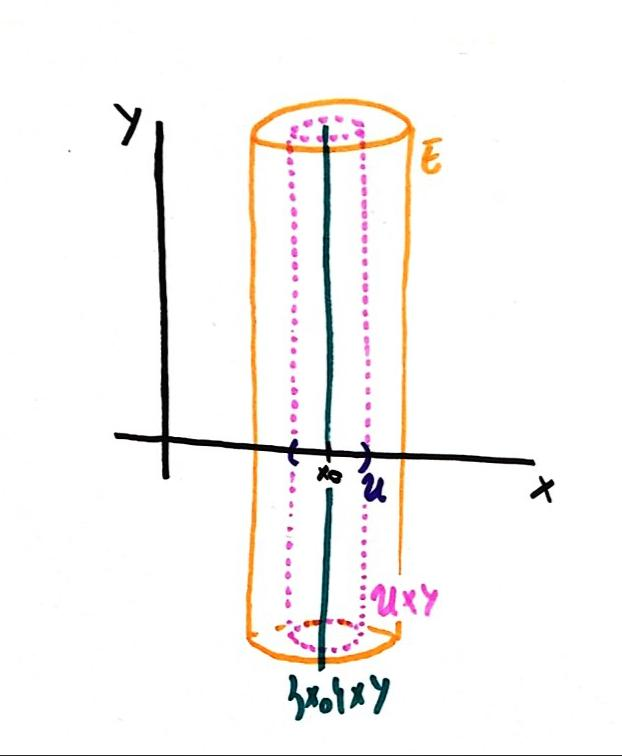
\includegraphics[scale = 0.3]{fotos_topo_1/lematub.jpeg}
\end{equation}

\begin{nota}
\label{nota:lematub} Si $Y$ no és compacte el lema és fals. Per exemple, siguin $X = Y = \mathbb{R}$, $x_0 = 0$ i sigui $E$ el complementari del conjunt $\{(x,y)\in\mathbb{R}^2\;:\;xy=1\}$. Aleshores no existeix un entorn $U$ del 0 a $\mathbb{R}$ com al lema.
\end{nota}

\begin{coro}
\label{coro:lematub} Amb les mateixes hipòtesis del lema, la projecció $p_X = X\times Y\rightarrow X$ és tancada.
\end{coro}
\begin{proof}
Sigui $T$ un tancat de $X\times Y$ i sigui $x_0\in X\setminus p_X(T)$. Per construcció, $X\times Y\setminus T$ és un obert que conté $\{x_0\}\times Y$ i, pel lema, existeix un obert $U$ tal que $x_0\in U$ i $U\times Y\subset X\times Y\setminus T$. Projectant sobre $X$: $U\subset X\setminus p_X(T)$. En conseqüència, $x_0$ és interior a $X\setminus p_X(T)$.
\end{proof}

\subsection{Producte de quasi-compactes}

\begin{ter}
\label{ter:productedespaisqc} Siguin $X_1,\ldots,X_n$ espais topològics. El producte $X_1\times \cdots\times X_n$ és quasi-compacte si i només si els espais $X_1,\ldots,X_n$ ho són.
\end{ter}
\begin{proof}
Si $X_1\times \cdots\times X_n$ és quasi-compacte, cada factor ho és aplicant a les projeccions la proposició anterior.

Per veure la implicació contrària, per inducció, és suficient tractar el cas $n = 2$. Sigui $\mathcal{A}=\{U_i\}_{i\in I}$ un recobriment obert de $X\times Y$. Fixat $x_0\in X$, $\mathcal{A}$ és també un recobriment obert de $\{x_0\}\times Y$ i, per tant, existeixen $i_1,\ldots,i_n\in I$ tals que $\{x_0\}\times Y\subset U_{i_1}\cup\cdots\cup U_{i_n}$. Aplicant el lema del tub (\ref{lema:lemadeltub})a $E = U_{i_1}\cup\cdots\cup U_{i_n}$ deduïm: per a tot punt $x_0\in X$ existeix un entorn obert $W_{x_0}$ de $x_0$ a $X$ tal que $W_{x_0}\times Y$ està recobert per un nombre finit d'elements de $\mathcal{A}$. Com que $\{W_{x_0}\}_{x_0\in X}$ és un recobriment de l'espai quasi-compacte $X$ obtenim que 
\begin{equation}
    \notag
    X = W_{x_1}\cup\cdots\cup W_{x_n}
\end{equation}
per a certs $x_1,\ldots,x_n\in X$. Ajuntant els oberts que per a cada $i=1,\ldots,n$, donen un recobriment finit de $W_{x_i}\times Y$ per elements de $\mathcal{A}$, obtenim un subrecobriment finit.
\end{proof}

\begin{ej}
\label{ej:producteqc} Alguns exemples:
\begin{enumerate}[(1)]
    \item $I = [0,1]$ és quasi-compacte
    \item $I^n\subset\mathbb{R}^n$ és quasi-compacte, ja que és $I\times I\times\cdots\times I$, $n$ vegades.
\end{enumerate}
\end{ej}

\begin{coro}
\label{coro:producteeq} Tot subconjunt tancat i afitat (o acotat) de $\mathbb{R}^n$ (amb $\tau_e$) és quasi-compacte.
\end{coro}
\begin{proof}
 Si $T\subseteq\mathbb{R}^n$ és afitat, existeix un interval $[a,b]\subset\mathbb{R}$ tal que $T\subset[a,b]^n$. Així $T$ és un tancat en un quasi-compacte, per tant és quasi-compacte. 
\end{proof}

\section{Espais compactes}

\begin{defi}
[Espais compactes]\label{def:espaiscompactes}\index{Espais compactes} Sigui $(X,\tau)$
\end{defi}

Recordem que un subespai tancat d'un espai quasi-compacte és quasi-compacte. En canvi, no és cert que un subespai quasi-compacte d'un espai topològic sigui tancat. Per exemple, sigui $X = \{1,2\}$ amb la topologia grollera. Aleshores $\{1\}$ és un subespai quasi-compacte, però no és tancat. La introducció de la propietat de separació permet tenir aquesta propietat en els espais compactes.

Veiem que ja vam afirmar a (\ref{prop:ent2qcimplicatancat}) que si $X$ és de Hausdorff, aleshores un subespai $A\subseteq X$ quasi-compacte és tancat. La hipòtesi de Hausdorff és necessària. Però jo pensava: cal que el subconjunt $A\subseteq X$ sigui de Hausdorff, a més de quasi-compacte? (és a dir, cal que sigui compacte?). Bé, doncs si $A$ és quasi-compacte i $X$ és de Hausdorff, com la propietat de Hausdorff és hereditària (\ref{prop:hausdorff2}), automàticament $A$ és de Hausdorff, ergo $A$ és compacte. Veiem doncs, que el següent teorema és, en realitat, el mateix teorema que (\ref{prop:ent2qcimplicatancat}). Tot i així, l'enunciaré perquè aquí (als apunts del Naranjo-Navarro) és una mica més precís.

\begin{prop}
\label{prop:compactedehausdorffestancat} Tot subconjunt compacte d'un espai de Hausdorff és tancat.
\end{prop}
\begin{proof}
 Amb l'observació que he fet al principi i la demostració de la proposició (\ref{prop:ent2qcimplicatancat}) ja tenim suficient.
\end{proof}

Una conseqüència de la proposició aquesta és la caracterització següent dels compactes de $\mathbb{R}^n$:

\begin{coro}
\label{coro:compactesiiacotatitancat} $X\subseteq\mathbb{R}^n$ és compacte si, i només si, $X$ és tancat i afitat.
\end{coro}
\begin{proof}
 Ja s'ha vist que si $X$ és tancat i afitat, aleshores és quasi-compacte al corol·lari (\ref{coro:producteeq}) i, en ser $\mathbb{R}^n$ de Hausdorff, per (\ref{prop:hausdorff2}) $X$ és compacte.
 
 Recíprocament, si $X$ és compacte és tancat per la proposició (\ref{prop:compactedehausdorffestancat}), i si $X$ no fos afitat, $\mathcal{A} = \{B_n(0)\cap X\}_{n\in\mathbb{N}}$ és un recobriment obert sense recobriment finit (això, pel contrarrecíproc, prova que $X$ és afitat).
\end{proof}

\begin{ej}
\label{ej:espaiscompactes}
Alguns exemples:
\begin{enumerate}[(1)]
    \item La esfera $S^n\subset \mathbb{R}^{n+1}$ és compacta.
    \item $\mathbb{R}^n$, amb $n>0$, els hiperplans de $\mathbb{R}^n$, la paràbola,... no són compactes.
\end{enumerate}
També a conseqüència de la proposició s'obté el corol·lari següent:
\end{ej}

\begin{coro}
\label{coro:fentreqcihausdorffestancada} Sigui $f:X\rightarrow Y$ una aplicació contínua entre espais topològics tals que $X$ és quasi-compacte i $Y$ és de Hausdorff. Aleshores $f$ és tancada.
\end{coro}
\begin{proof}
 Sigui $T$ un tancat de $X$. Com que $X$ és quasi-compacte, per (\ref{prop:tancatesqc}) $T$ és quasi-compacte. Com $f$ és contínua, per (\ref{prop:preservaciodelaqcperappcontinues}) $f(T)$ és quasi-compacte. Com $Y$ és de Hausdorff, $f(T)$ és tancat. Aleshores $f$ és tancada.
\end{proof}

És clar que la compacitat és una propietat invariant per homeomorfismes i, per tant, podem utilitzar el corol·lari anterior per obtenir que certs espais topològics no són homeomorfs. Per exemple:
\begin{enumerate}[(1)]
    \item L'el·lipse i la paràbola no són homeomorfes.
    \item El cilindre obert i l'esfera no són homeomorfs.
    \item $(0,1)$ i $[0,1]$ no són homeomorfs.
\end{enumerate}

\begin{prop}
\label{prop:totespaicompacteesnormal} Tot espai topològic compacte és normal.
\end{prop}
\begin{proof}
 Siguin $F_1,F_2$ dos tancats disjunts d'un espai compacte $X$. Com que $F_1$ és compacte, per a cada punt $x\in F_2$ existeixen, pel lema, oberts disjunts $U_x$ i $V_x$ tals que $F_1\subset U_x$ i $x\in V_x$. Aleshores 
 \begin{equation}
     \notag
     F_2\subset\bigcup_{x\in F_1} V_x
 \end{equation}
 i, per la compacitat de $F_2$, existeixen $x_1,\ldots,x_n\in X$ tals que $F_2\subset V_{x_1}\cup\cdots\cup V_{x_n}$. Definint $V = V_{x_1}\cup\cdots\cup V_{x_n}$ i $U = U_{x_1}\cup\cdots\cup U_{x_n}$, obtenim dos oberts disjunts tals que $F_1\subset U$ i $F_2\subset V$.
\end{proof}

\section{Espais mètrics compactes}

Tot espai mètric dóna lloc, de manera natural, a un espai topològic (veure topologia usual (\ref{def:topologiausual})). Així doncs, quan ens referim a espais mètrics compactes estem tractant la relació entre la compacitat a espais mètrics i la compacitat als espais topològics als que donen pas. El Teorema de Heine-Borel (\ref{ter:teoremadeheineborel}) caracteritza els subconjunts de $\mathbb{R}^n$ que són compactes, identificant-los amb els tancats i acotats. Per tant, és un teorema que es refereix \textbf{únicament a espais topològics amb la topologia euclidiana}.

\begin{ej}
\label{ej:espaimetriccompacte} $(\mathbb{R},d)$ espai mètric amb $d$ distància euclidiana. El subconjunt $S = (0,1)\subset\mathbb{R}$ no és compacte en $\mathbb{R}$. Per veure-ho, hem de trobar un recobriment obert $\mathcal{F}$ de $S$ que no tingui un subrecobriment finit.  Considerem el següent recobriment obert de $S$:
\begin{equation}
    \notag
    \mathcal{F} = \left\{\left(0,1-\frac{1}{n}\right)\;:\;n\in\mathbb{Z},\;n\geq 1\right\} = \left\{\left(0,\frac{1}{2}\right),\left(0,\frac{2}{3}\right),\left(0,\frac{3}{4}\right),\cdots\right\}. 
\end{equation}
Clarament $\mathcal{F}$ és un subrecobriment infinit de $(0,1)$. A més,
\begin{equation}
    \notag
    (0,1)\subseteq\bigcup_{k=2}^\infty \left(0,1-\frac{1}{k}\right) .
\end{equation}
Sigui $\mathcal{F}^*$ un subconjunt finit de $\mathcal{F}$ que conté $p$ elements. Aleshores 
\begin{equation}
    \notag
    \mathcal{F}^* = \left\{\left(0,1-\frac{1}{n_1}\right),\ldots,\left(0,1-\frac{1}{n_p}\right)\right\}
\end{equation}
Sigui $n^* = \max\{n_1,\ldots,n_p\}$. Donada la naturalesa dels oberts de $\mathcal{F}$, 
\begin{equation}
    \notag
    \bigcup_{k=1}^p\left(0,1-\frac{1}{n_k}\right)\subseteq \left(0,1-\frac{1}{n^*}\right)
\end{equation}
Però per a que $(0,1)\subseteq (0,1-1/n^*)$ necessitem $1\leq 1-1/n^*$ i $n^*\in\mathbb{N}$, per tant $n^*>0$, és a dir, $1/n^*>0$, aleshores $1-1/n^*>1$. Per tant qualsevol subconjunt $\mathcal{F}^*$ finit de $\mathcal{F}$ no pot cobrir a tot $S = (0,1)$. Per tant, no és compacte.
\end{ej}

\subsection{Espais seqüencialment compactes}

En aquest apartat $(X,d)$ és un espai mètric. Compararem la noció de compacitat en espais mètrics amb la noció següent associada a successions.

\begin{defi}[Espais mètris seqüencialment compactes]
\label{def:espaisequencialmentcompactes}\index{Espais mètrics seqüencialment compactes} $(X,d)$ és \textit{seqüencialment compacte} (o compacte per successions) si per a tota successió $(x_n)_{n\in\mathbb{N}}$, amb $x_n\in X$, existeix una successió parcial $(x_{n_k})_{k\in\mathbb{N}}$ que és convergent.\footnote{Recordem que si $(x_n)_n$ és una successió, definíem una successió parcial $(x_{n_k})_k$ com una subsuccessió tal que $(n_k)_k$ és estrictament creixent. Es denotava per $(x_{n_k})_k\vdash (x_n)_n$.}
\end{defi}

L'objectiu és veure que, en espais mètrics, compacte i seqüencialment compacte signifiquen el mateix. Necessitem alguns resultats previs. Tot això no ho acabo d'entendre i, més encara, no entenc per què ho fem a topologia. Així doncs, ho copiaré tal qual està als apunts del Naranjo-Navarro.

\begin{defi}
[Diàmetre]\label{def:diametre}\index{Diàmetre} Sigui $A\subset X$. El \textit{diàmetre} es defineix com 
\begin{equation}
    \notag
    diam(A) = \sup_{x,y\in A}\{d(x,y)\}. 
\end{equation}
és un element de $\mathbb{R}\cup\{\infty\}$.
\end{defi}
\begin{ej}
\label{ej:diametre} Exemples de diàmetres:
\begin{enumerate}[(1)]
    \item $diam(\mathbb{R}) = \infty$.
    \item $diam([a,b]) = diam((a,b)) = b-a$.
    \item En general, el diàmetre d'una bola de radi $r$ en un espai mètric és menor o igual a $2r$.
    \item Si $A$ és compacte, com que $d$ és contínua, $d(A\times A)$ és un compacte de $\mathbb{R}$ i per tant $diam(A)<\infty$.
\end{enumerate}
\end{ej}

\begin{defi}
[Nombre de Lebesgue]\label{def:nombredelebesgue}\index{Nombre de Lebesgue} Sigui $\mathcal{A} = \{U_i\}_{i\in I}$ un recobriment obert de $X$. Diem que $\lambda\in\mathcal{R}$, $\lambda>0$ és un número de Lebesgue per al recobriment $\mathcal{A}$ si per a tot subconjunt $A\subset X$ amb $diam(A)<\lambda$ existeix $i\in I$ tal que $A\subset U_i$.
\end{defi}

\begin{prop}
\label{prop:existeixnumerolebesgue} Si $X$ és seqüencialment compacte per a tot recobriment obert d'$X$ existeix un número de Lebesgue.
\end{prop}
\begin{proof}
 Raonem per absurd. Suposem que no existeix cap número de Lebesgue per a un recobriment obert $\{U_i\}_{i\in I}$. Per a tot natural $n$ existirà un subconjunt $A$ no contingut en cap obert $U_i$ tal que $diam(A)<1/n$. Observem que si $x_n\in A$, tenim, per definició del diàmetre, que $B_{1/n}(x_n)\supset A$. En particular, cap obert del recobriment conté la bola $B_{1/n}(x_n)$.
 
 Sigui $x$ el límit d'una parcial convergent de la successió $(x_n)_{n\in\mathbb{N}}$ i sigui $j\in I$ tal que $x\in U_j$. Si $m$ és prou gran, $B_\frac{1}{m}(x)\subset U_j$. Un element $x_n$ de la parcial convergent tal que $n>2m$ i $d(x_n,x)<\frac{1}{2m}$ verifica, per a tot $y\in B_{1/n}(x_n)$:
 \begin{equation}
     \notag
     d(x,y)\leq d(y,x_n)+d(x_n,x)\leq \frac{1}{n}+\frac{1}{2m}< \frac{1}{2m}+\frac{1}{2m}= \frac{1}{m}
 \end{equation}
 Per tant $B_{1/n}(x_n)\subset B_{1/m}(x)\subset U_i$ absurd.
\end{proof}

Veiem ara el teorema central de la secció:

\begin{ter}
\label{ter:compactesiisequencialmentcompacte} Sigui $(x,d)$ un espai mètric. Són equivalents
\begin{enumerate}[(a)]
    \item $X$ és compacte.
    \item $X$ és seqüencialment compacte.
\end{enumerate}
\end{ter}
\begin{proof}
\fbox{$(a)\Rightarrow(b)$} Sigui $(x_n)_{n\in\mathbb{N}}$ una successió a $X$, i posem $F_n = \{x_n,x_{n+1},\ldots\}$. Primer provarem que $\cap_n \overline{F_n}\not=\emptyset$. Per absurd, suposem que  $\cap_n\overline{F_n}=\emptyset$. Per la compacitat $\overline{F_{n_1}}\cap\cdots\cap \overline{F_{n_k}}=\emptyset$. Això porta a una contradicció: si $m = \max\{n_1,\ldots,n_k\}$, aleshores
\begin{equation}
    \notag
    \emptyset\not= F_m\subset F_{n_1}\cap \cdots\cap F_{n_k}\subset \overline{F_{n_1}}\cap\cdots\cap \overline{F_{n_k}}.
\end{equation}
Sigui ara $a\in\cap_n \overline{F}_n$. Per ser adherent a $F_m$ tenim que
\begin{equation}
    \notag
    B_{\frac{1}{m}}(a)\cap F_m\not=\emptyset.
\end{equation}
Considerem $X_{n_m}$ en aquesta intersecció, i considerem la successió $\{x_{n_m}\}_{n\in\mathbb{N}}$. Per a tot $m$, $d(x_{n_m},a)<\frac{1}{m}$. Per tant, $\displaystyle\lim_{m\rightarrow\infty}x_{n_m}=a$.

\fbox{$(b)\Rightarrow(a)$} Sigui $U = \{U_i\}_{i\in I}$ un recobriment obert de $X$. Per la proposició, existeix un número de Lebesgue $\lambda$ per a aquest recobriment. Sigui $0<\lambda_0<\frac{\lambda}{2}$. Aleshores, per a tot $x\in X$, existeix $j\in I$ tal que $B_{\lambda_0}(x)\subset U_j$. Sigui $x_1\in X$ arbitrari i sigui $U_1$ un obert del recobriment tal que $B_{\lambda_0}(x_1)\subset U_1$. De la mateixa manera seleccionem per a $x_2\in X\setminus U_1$ un obert $U_2$ tal que $B_{\lambda_0}(x_2)\subset U_2$. Suposant que $U$ no admet un subrecobriment finit, podem repetir aquest procés indefinidament, fins a construir una successió $(x_n)_{n\in\mathbb{N}}$ d'elements de $X$ verificant la propietat següent: per a tot $n$, si $x_m\in B_{\lambda_0}(x_n)$, aleshores $m=n$.

En particular, per a tot $n,m$ diferents $d(x_n,x_m)\geq \lambda_0$. És clar que una successió amb aquesta propietat no pot tenir una successió parcial convergent, absurd.
\end{proof}

\begin{defi}
[Aplicació uniformement contínua]\label{def:appuniformementcontinua}\index{Aplicació uniformement contínua entre espais mètrics} Una aplicació $f:X\rightarrow Y$ entre dos espais mètrics és \textit{uniformement contínua} si per a tot $\varepsilon>0$ existeix $\delta>0$ tal que per a tot $x\in X$, $f(B_\delta(x))\subset B_\varepsilon(f(x))$ (és a dir, $\delta$ no depèn  de $x$).
\end{defi}

\begin{prop}
\label{prop:uniformementcontinua} Si $f:X\rightarrow Y$ és una aplicació contínua entre espais mètrics i $X$ és compacte, aleshores $f$ és uniformement contínua.
\end{prop}
\begin{proof}
Considerem el recobriment obert de $X$: $\{f^{-1}(B_{\varepsilon/2}(y))\}_{y\in Y}$. Com que $X$ és compacte existeix un número de Lebesgue $\lambda$ per a aquest recobriment. Tenim així que, per a tot $x\in X$, existeix $y\in Y$ tal que 
\begin{equation}
    \notag
    f(B_{\lambda/2}(x))\subset B_{\varepsilon/2}(y).
\end{equation}
En particular, $f(x)\in B_{\varepsilon/2}(y)$, i, per la desigualtat triangular, es té que $B_{\varepsilon/2}(y)\subset B_\varepsilon(f(x))$.

Definint $\delta = \lambda/2$ arribem a 
\begin{equation}
    \notag
    f(B_\delta(x))\subset B_{\varepsilon/2}(y)\subset B_\varepsilon(f(x)).
\end{equation}
\end{proof}

\section{El lema de Heine-Borel}

Per completar el tema, afegim aquí una demostració del teorema de Heine-Borel.

\begin{ter}
[Heine-Borel]\label{ter:teoremadeheineborel} Tot subconjunt tancat i afitat de $\mathbb{R}$ és quasi compacte.
\end{ter}
\begin{proof}
Sigui $X\subseteq\mathbb{R}$ tancat i afitat. En particular, existeixen $a,b\in\mathbb{R}$, $a<b$, tals que $X\subset [a,b]$. Com que un tancat és quasi compacte, és suficient veure que $[a,b]$ ho és. Sigui $\mathcal{A}$ un recobriment obert de $[a,b]$. Definim
\begin{equation}
    \notag
    \mathcal{C} = \{x\in(a,b]\;:\;\text{$[a,x]$ pot ser recobert per un nombre finit d'oberts de $\mathcal{A}$}\}
\end{equation}
$\mathcal{C}$ no és buit, ja que donat $U\in\mathcal{A}$ tal que $a\in U$, existirà un $y'>a$ tal que $[a,y')\subset U$, ja que els intervals oberts són base. Aleshores, per a qualsevol $a<y<y'$, tindrem $[a,y]\subset U$ i, per tant, $y\in\mathcal{C}$. Sigui $c = \sup\mathcal{C}$. La resta de la demostració consisteix a provar que $c\in\mathcal{C}$ i que $c = b$.

Veiem primer que $c\in\mathcal{C}$, és a dir, que $[a,c]$ es pot recobrir per un nombre finit d'elements de $\mathcal{A}$. Sigui $V\in\mathcal{A}$ tal que $c\in V$. Com que $c>a$, existeix $a<c'<c$ tal que $(c',c]\subset V$. Com $c$ és el suprem de $\mathcal{C}$, existeix $x\in\mathcal{C}\cup (c',c]$. Aleshores $[a,c]=[a,x]\cup[x,c]$. Per definició de $\mathcal{C}$, $[a,x]$ es pot recobrir per un nombre finit d'elements de $\mathcal{A}$ i $[x,c]\subset V\in\mathcal{A}$.

Finalment provem que $c = b$. Si $c<b$, agafant $V\in\mathcal{A}$ com abans, trobem un $d$ tal que $c<d\leq b$ i $[c,d]\subset V$. Com que $[a,d] = [a,c]\cup[c,d]$ i $c\in\mathcal{C}$, tenim que $d\in\mathcal{C}$, la qual cosa contradiu que $c$ sigui el suprem.
\end{proof}









\section{Espais localment compactess}

El propòsit d'aquest capítol és construir espais compactes (quasi-compactes + Hausdorff) a partir d'altres no compactes. Aquest procés no és únic i aquí ens concentrem en el cas que únicament s'afegeix un punt a l'espai inicial per obtenir un espai compacte. La construcció gaudeix de propietats especialment agradables quan l'espai inicial verifica condicions de caire local, que són estudiades en el primer apartat.

\begin{defi}
[Localment compacte]\index{Espai localment compacte}\index{Localment compacte}\label{def:localmentcompacte} Sigui $(X,\tau)$ un espai topològic. Diem que $X$ és \textit{localment compacte} si és de Hausdorff i tot punt de $X$ té un entorn compacte.
\end{defi}

\begin{ej}
\label{ej:localmentcompacte1} $\mathbb{R}^n$ és localment compacte (amb la topologia euclidiana). En efecte, clarament és de Hausdorff pel que ja vam veure al capítol de Propietats de separació (\ref{ej:hausdorff2}). Veiem que tot punt $x\in\mathbb{R}^n$ té un entorn compacte. Sigui $x\in\mathbb{R}^n$ un punt qualsevol. Prenem $r>0$ i la bola tancada $\overline{B(x,r)}$ és un entorn compacte de $x$. Com ja vam veure, a tot espai topològic amb la topologia usual, un subespai era compacte si era tancat i acotat. Aleshores, com $\overline{B(x,r)}$ és tancada i acotada, és compacte. Observem, però, que $\mathbb{R}^n$ no és compacte per sí sol. Així doncs, tenim un contraexemple que localment compacte no implica compacte.
\end{ej}

\begin{ej}
\label{ej:localmentcompacte2} Sigui $X$ un conjunt dotat de la topologia discreta. Aleshores, tenim que $\forall x\in X$, $\{x\}$ és un conjunt compacte ($X$ és de Hausdorff, veure \ref{ej:hausdorff3}) i és un entorn de $x$. Aleshores, $X$ és un espai topològic localment compacte. Notem que si $X$ és finit o infinit però numerable, aleshores és compacte. Però si és infinit no numerable, no.
\end{ej}

\begin{prop}
\label{prop:compacteimplicalocalmentcompacte} Tot espai compacte és localment compacte.
\end{prop}
\begin{proof}
$\forall x\in X$, podem prendre $X$ com a entorn de $x$ i $X$ és compacte, per tant tot punt té un entorn compacte.
\end{proof}

\begin{prop}
\label{prop:tancatlocalmentcompacte} Sigui $X$ un espai topològic localment compacte i sigui $A\subset X$ un tancat. Aleshores $A$ és localment compacte.
\end{prop}
\begin{proof}
Sigui $x\in A$ i sigui $K$ un entorn compacte de $x$ en $X$. Aleshores $K\cap A$ és un entorn de $x$ a $A$ i, en ser $K\cap A$ un tancat del compacte $K$, és compacte.
\end{proof}

La mateixa propietat és certa per a subconjunts oberts. Aquest fet s'obté com a conseqüència del fet següent:

\begin{prop}
\label{prop:localmentcompactebaseentorns} Tot punt d'un espai localment compacte té una base d'entorns compactes.
\end{prop}
\begin{proof}
Sigui $x\in X$ i sigui $U$ un entorn obert de $x$. Per hipòtesis, existeix un entorn compacte $K$ de $x$. Aleshores $U\cap K$ és un obert de $K$ i, per tant, $T = K\setminus U\cap K$ és un tancat de $K$ i $x\not\in T$. Com que $K$ és normal, existeixen oberts de $K$, $W_x$ i $W_T$ tals que $x\in W_x$ i $T\subset W_T$ i $W_x\cap W_T = \emptyset$. Per tant, $K\setminus W_T$ és un entorn de $x$ a $K$. Com que $K$ és un entorn de $x$, també $K\setminus W_T$ és entorn de $x$ a $X$. Finalment observem que $K\setminus W_T$ és un tancat en un compacte, per tant és compacte i $K\setminus W_T\subset K\setminus T\subset U$.
\end{proof}

\begin{defi}
[Localment]\index{Localment}\label{def:localment} Sigui $P$ una propietat dels espais topològics, com per exemple $T_1$, o compacte,... Diem que un espai topològic és \textit{localment} $P$ si tot punt de $X$ té una base d'entorns verificant $P$.
\end{defi}

La proposició anterior ens diu que en espais $T_2$ la definició d'espai localment compacte que hem donat al principi coincideix amb la que hauríem d'haver donat seguint aquesta definició general de ``localment $P$''.

Com havíem dit, tot obert d'un espai localment compacte és localment compacte, i ara ho veiem:

\begin{coro}
\label{coro:localmentcompacteobert} Un obert d'un espai localment compacte és localment compacte.
\end{coro}
\begin{proof}
Sigui $X$ localment compacte i $U\subset X$ un obert, i $x\in U$. Per la proposició (\ref{prop:localmentcompactebaseentorns}) existeix un entorn compacte $K$ de $x$ tal que $x\in K\subset U$. Per tant, $U$ és localment compacte.
\end{proof}

\begin{prop}
\label{prop:productedelocalmentcompactes} El producte de dos espais topològics localment compactes és localment compacte.
\end{prop}
\begin{proof}
Siguin $X,Y$ localment compactes. Com que el producte d'espais de Hausdorff és de Hausdorff, $X\times Y$ és de Hausdorff, per (\ref{prop:hausdorff2}). Sigui $(x,y)\in X\times Y$ i siguin $K_x, K_y$ entorns compactes de $x,y$ respectivament. Aleshores $K_x\times K_y$ és un entorn compacte de $(x,y)$.
\end{proof}





\section{Compactificacions} 

Considerem un espai topològic $(X,\tau)$. Aleshores, $X$ pot no ser compacte, depenent de la topologia $\tau$. Si $X$ no és compacte, potser volem construir un espai topològic compacte a partir de $X$ que conservi tot el possible la topologia $\tau$. El que farem serà estudiar espais topològics compactes que continguin a $X$ com a subespai dens (és a dir, que $\overline{X}$ serà tot l'espai)

La definició que donen a \cite{mathonline} és la següent: donat $(X,\tau)$ un espai topològic que no és compacte, una compactificació és un altre espai espai topològic $(Y,\tau')$ tal que $X$ és subespai de $Y$ i tal que $X$ és dens en $Y$, és a dir, $\overline{X}=Y$. Jo posaré la definició que dóna els apunts \cite{naranjo}, encara que al cap i a la fi arribem a dos conceptes equivalents.

\begin{defi}
[Compactificació]\index{Compactificació}\label{def:compactificacio} Sigui $X$ un espai topològic. Una \textit{compactificació} de $X$ és un espai topològic compacte $X^*$ i una aplicació contínua $h:X\rightarrow X^*$ tal que $X\rightarrow h(X)$ és homeomorfisme i $\overline{h(X)} = X^*$.
\end{defi}

\begin{ej}
\label{ej:compactificacions} Exemples de compactificacions:
\begin{enumerate}[(1)]
    \item $X = (0,1)$, $X^* = [0,1]$ i $h:X\hookrightarrow X^*$ la inclusió.
    \item $X = \mathbb{R}^n$, $X^* = S^n$ i $h:\mathbb{R}^n\rightarrow S^n\setminus\{p\}\hookrightarrow S^n$ la inversa de la projecció estereogràfica.
    \item Com que $(0,1)$ és homeomorf a $\mathbb{R}$, l'exemple anterior ens dona una compactificació diferent de l'exemple 1 per al $(0,1)$.
    \item $X = \mathbb{N}$, $X^*=\{0\}\cup\{1/n \;:\;n\in\mathbb{N}\}$ i $h(n) = 1/n$.
\end{enumerate}
\end{ej}


\subsection{Compactificació per un punt o d'Alexandroff}

\begin{defi}
[Compactificació d'Alexandroff]\index{Compactificació d'Alexandroff}\index{Compactificació per un punt}\index{Alexandroff} Una compactificació $h:X\rightarrow X^*$ és d'\textit{Alexandroff} o \textit{per un punt} si $X^*\setminus h(X)$ és un punt. Aquest punt el denotem per $\infty$. De vegades posem $X^* = X_\infty$.
\end{defi}

És a dir, la compactificació d'Alexandroff consisteix a agafar l'espai topològic corresponent i afegir-hi un punt que el fa compacte.

Per demostrar l'existència d'una tal compactificació definim sobre $X^* = X\cup\{\infty\}$, on $\infty$ és un objecte arbitrari fora de $X$, la topologia següent:
\begin{equation}
    \notag
    \tau^* = \{U = X^*\setminus C\;:\; C\subset X\;\text{compacte}\}\cup\tau_X
\end{equation}
on $\tau_X$ és la topologia que hi ha definida sobre $X$.

\begin{lema}
\label{lema:topologiacompactificacio} $\tau^*$ és una topologia sobre $X^*$.
\end{lema}
\begin{proof}
Demostrem els tres punts de la definició de topologia.
\begin{enumerate}[(i)]
    \item $\emptyset\in\tau_X\subset\tau^*$ i com $\emptyset$ és compacte, $X^*\setminus \emptyset = X^*\in\tau^*$.
    \item Sigui $\{U_i\}_{i\in I}$ una família d'elements de $\tau^*$. Si per a tot $i$, $U_i\in\tau_X$, tenim que $\bigcup_{i\in I} U_i \in\tau_X$ i ja hem acabat. En cas contrari, suposem que $I = I_1\cup I_2$ de manera que
    \begin{equation}
        \notag
        I_1 = \{i\in I\;:\;U_i\in \tau_X\},\qquad I_2 = \{i\in I\;:\;U_i = X^*\setminus C_i,\;\text{on $C_i\subset X$ és compacte}\}. 
    \end{equation}
    Aleshores,
    \begin{equation}
        \notag
        \bigcup_{i\in I}U_i = \left(\bigcup_{i \in I_1 U_i}\right)\cup\left(\bigcup_{i\in I_2}(X^*\setminus C_i)\right) =
    \end{equation}
    \begin{equation}
        \notag
        \left(\bigcup_{i\in I_1}U_i\right)\cup\left(X^*\setminus \bigcup_{i\in I_2}C_i\right) = X^*\setminus\left[\left(\bigcup_{i\in I_2}C_i\right)\setminus\left(\bigcup_{i\in I_1}U_i\right)\right]
    \end{equation}
    Com que $I_2\not=\emptyset$, el conjunt $\bigcup_{i\in I_2}C_i\setminus \bigcup_{i\in I_1}U_i$ és compacte i, per tant, $\bigcup_{i\in I}U_i\in \tau^*$.
    \item És suficient veure que la intersecció de dos elements de $\tau^*$ és de $\tau^*$. Si $U$ i $V$ són dos oberts de $\tau_X$, aleshores $U\cap V\in\tau_X\subset \tau^*$. Si $U = X^*\setminus C$, amb $C\subset X$ compacte i $V\in\tau_X$, aleshores 
    \begin{equation}
        \notag
        U\cap V = (X^*\setminus C)\cap V = (X\setminus C)\cap V \in\tau_X\subset \tau^*
    \end{equation}
    Finalment si $U = X^*\setminus C_1$ i $V = X^*\setminus C_2$, amb $C_1,C_2\subset X$ compactes de $X$, aleshores 
    \begin{equation}
        \notag
        (X^*\setminus C_1)\cap(X^*\setminus C_2) = X^*\setminus(C_1\cup C_2)\in\tau^*
    \end{equation}
    ja que la unió finita de compactes és compacte (veure exercicis de compacitat).
\end{enumerate}
\end{proof}

Demostrem ara que, en efecte, la compactificació d'Alexandroff és una compactificació.

\begin{ter}
\label{ter:compactificaciodalexandroff} El parell $(X^*,h)$ és una compactificació de $X$.
\end{ter}
\begin{proof}
Primer demostrem que $X^*$ és quasi-compacte. Sigui $\{U_i\}_{i\in I}$ un recobriment de $X^*$. Recordem $X^* = X\cup\{\infty\}$, per tant $\exists i_0\in I$ tal que $\infty\in U_{i_0}$. Existeix un compacte $K$ tal que $U_{i_0} = X^*\setminus K$ (perquè l'element $U_{i_0}$ és un element de $\tau^*$ i no de $\tau_X$ perquè conté el $\infty$). Aleshores
\begin{equation}
    \notag
    \{K\cap U_i\}_{i\in I\setminus\{i_0\}} 
\end{equation}
ens dóna un recobriment obert de $K$. Siguin $i_1,\ldots,i_n\in I$ tals que
\begin{equation}
    \notag
    K = (K\cap U_{i_1})\cup\cdots\cup(K\cap U_{i_n}).
\end{equation}
Així, $X^* = U_{i_0}\cup U_{i_1}\cup\cdots\cup U_{i_n}$.

Per veure que $X^*$ és de Hausdorff només cal veure que $\infty$ se separa de tot punt $x\in X$. Sigui $K$ un entorn compacte de $x$, i sigui $U\in\tau_X\subset \tau^*$ tal que $x\in U\subset K$. Aleshores, $V = X^*\setminus K$ és un entorn obert del punt $\infty$ i $U\cap V = \emptyset$.

Observem que $h$ és oberta, atès que $\tau_X\subset\tau^*$. Per tant, $h:X\rightarrow h(X)$ és un homeomorfisme.

Finalment, provem que $\overline{h(X)} = X^*$. Atès que $X$ no és compacte, $h(X)$ no és tancat. Per tant, $h(X)\varsubsetneq \overline{h(X)}$ la qual cosa obliga a tenir $\overline{h(X)} = X^*$.
\end{proof}

\begin{prop}
\label{prop:unicitatdalexandroff} Sigui $(X^+,g)$ una altra compactificació de $X$ tal que $g(X)$ és un obert. Aleshores, existeix $f:X^+\rightarrow X^*$ contínua tal que $X\overset{g}{\longrightarrow} X^+\overset{f}{\longrightarrow X^*}$ és $h$ i $f(X^+\setminus g(X))=\{\infty\}$.

En particular, si $X^+$ és una altra compactificació per un punt, $f$ és un homeomorfisme
\end{prop}
\begin{proof}
Com a aplicació de conjunts $f$ està determinada per les condicions demanades:
\begin{equation}
    \notag
    \begin{array}{lll}
        \text{si} & a=g(x)\in g(X)\subset X^*, & f(a) = h(x) \\
        \text{si} & a\in X^*\setminus g(X), & f(a)=\infty.
    \end{array}
\end{equation}
Veiem que $f$ és contínua: si $U\subset \tau_X$, aleshores $f^{-1}(U) = g(h^{-1}(U))$. Com que $g:X\rightarrow g(X)$ és un homeomorfisme i $g(X)\subset X^+$ és un obert, tenim que $f^{-1}(U)$ és un obert. Si $U = X^*\setminus C$, on $C\subset X$ és un compacte:
\begin{equation}
    \notag
    f^{-1}(U) = X^+\setminus f^{-1}(C)=X^*\setminus g(h^{-1}(C)).
\end{equation}
Com que $g(h^{-1}(C))$ és compacte a $X^+$, és tancat i, per tant, el seu complementari és obert.
\end{proof}

\begin{ej}
\label{ej:alexandroff} Considerem la recta real $\mathbb{R}$ i el cercle unitat amb el punt $(0,1)$ extret: $S^1\setminus\{(0,1)\}$. Aleshores $S^1\setminus\{(0,1)\}$ és homeomorf a $\mathbb{R}$ a través del que es coneix com a projecció estereogràfica (veure apèndix)
\begin{equation}
    \notag
    f:S^1\setminus\{(0,1)\}\longrightarrow\mathbb{R},\quad f(x,y) = \frac{x}{1-y}.
\end{equation}
Per a tot punt $(x,y)\in S^1\setminus\{(0,1)\}$ el valor de $f(x,y)$ serà la intersecció de la línia que passa pel $(0,1)$ i $(x,y)$ amb l'eix $x$.
\begin{equation}
    \notag
    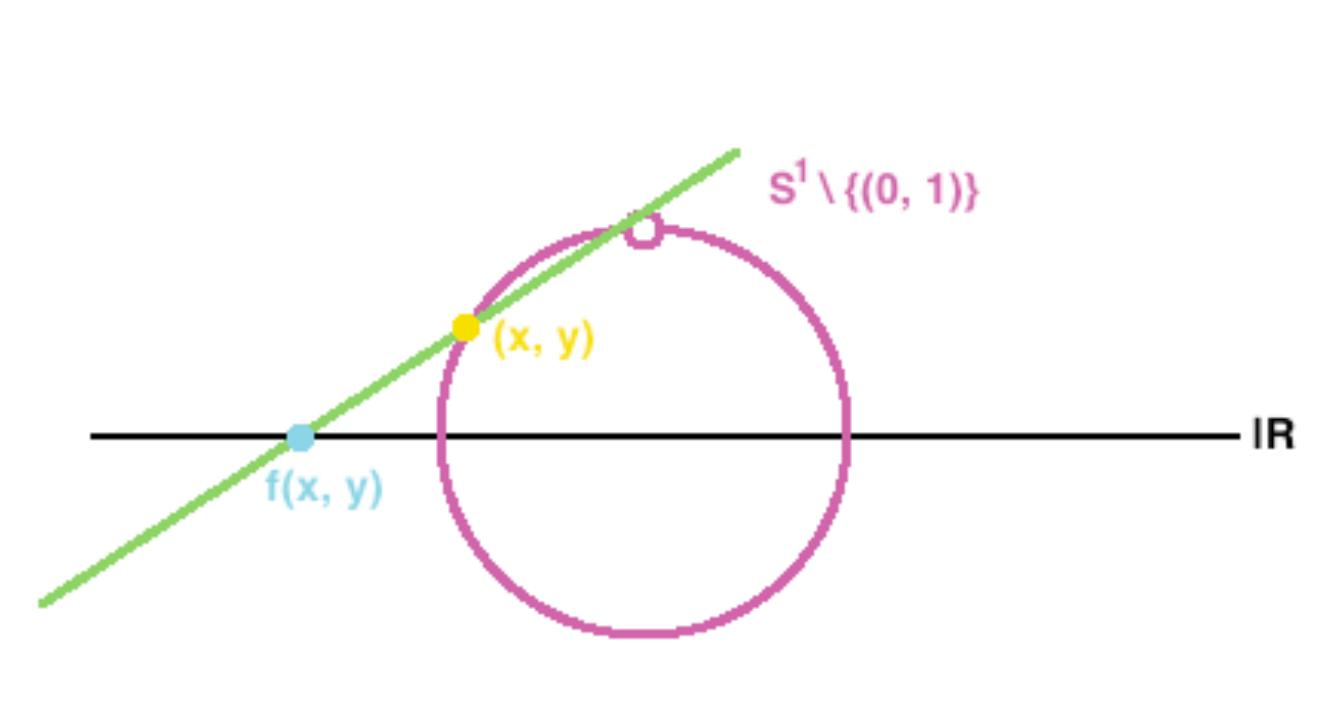
\includegraphics[scale = 0.3]{fotos_topo_1/ejemploalexandroff1.jpeg}
\end{equation}

Si pensem en el punt $\infty$ com el punt final de la recta numèrica (equivalent al punt que falta $(0,1)$) aleshores podem construir la compactificació d'Alexandroff de $\mathbb{R}$ com $(R^*,\tau^*)$, on $\mathbb{R}^* = \mathbb{R}\cup\{\infty\}$ i els oberts de $\mathbb{R}^*$ són de dos tipus:
\begin{enumerate}[1)]
    \item El primer tipus són els ``oberts normals'' de $\mathbb{R}$
    \begin{equation}
        \notag
        \includegraphics[scale = 0.3]{fotos_topo_1/ejemploalexandroff2.jpeg}
    \end{equation}
    \item El segon tipus d'oberts són els complementaris de tancats i compactes de $\mathbb{R}$
    \begin{equation}
        \notag
        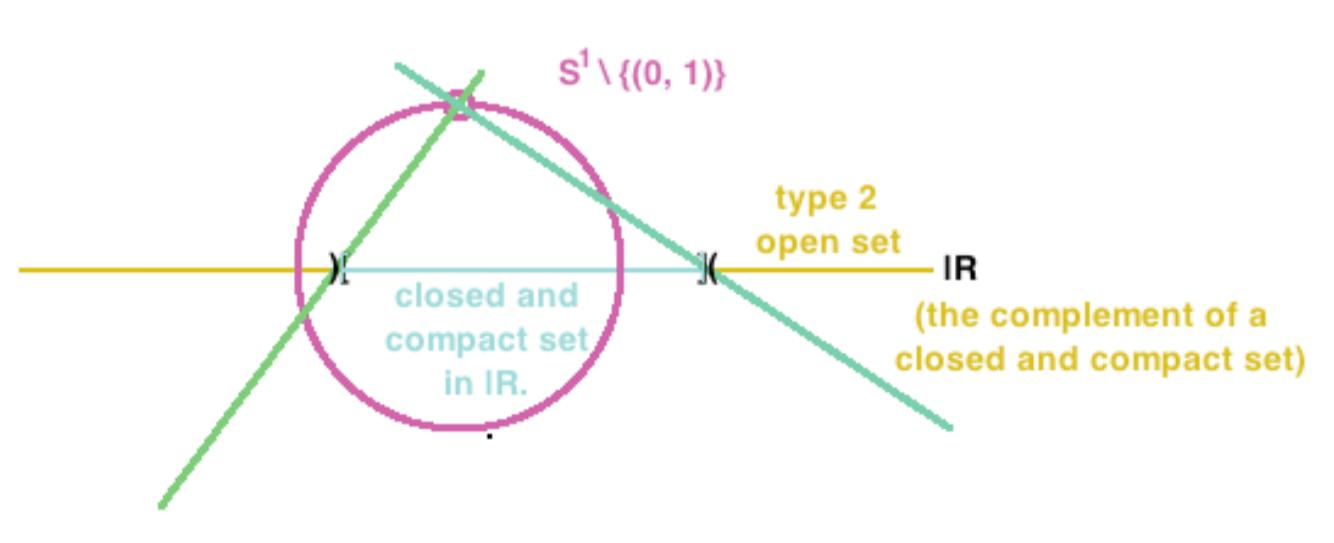
\includegraphics[scale = 0.3]{fotos_topo_1/ejemploalexandroff3.jpeg}
    \end{equation}
\end{enumerate}
\end{ej}

\begin{prop}
\label{prop:compactificatalexandroffhomeomorfisme} Siguin $X$ i $Y$ dos espais topològics i $X_\infty$, $Y_\infty$ els seus compactificats d'Alexandorff. Si $X\cong Y$, aleshores $X_\infty\cong Y_\infty$. 
\end{prop}
\begin{proof}
Si $f:X\rightarrow Y$ és un homeomorfisme, definim l'aplicació $f_\infty:X_\infty\rightarrow Y_\infty$ com
\begin{equation}
    \notag
    f_\infty(x) = \left\{
    \begin{array}{rcl}
        f(x), & \text{si} & x\not=\infty_X \\
        \infty_Y, & \text{si} & x=\infty_X
    \end{array}
    \right.
\end{equation}
i clarament és un homeomorfisme.
\end{proof}




\end{document}